%This LaTeX document was compiled in Overleaf
\documentclass[12pt]{article}
\usepackage[utf8]{inputenc}
\usepackage{tikz}
\usetikzlibrary{trees}
\usepackage{geometry}
\usepackage{pifont}
\usepackage{enumitem}
\usepackage{graphicx}
\usepackage[hidelinks]{hyperref}
\usepackage[defaultfam,tabular,lining]{montserrat} %% Option 'defaultfam'
%% only if the base font of the document is to be sans serif
%if the compiler used doesn't automatically support the Montserrat font,
%here's the link to the directory: https://www.ctan.org/tex-archive/fonts/montserrat/
\usepackage[T1]{fontenc}
\renewcommand*\oldstylenums[1]{{\fontfamily{Montserrat-TOsF}\selectfont #1}}
\geometry{a4paper, portrait, left=1.5cm, right=1.5cm, top=2cm,bottom=2cm}
\makeatletter
\renewcommand\@dotsep{1400}   
\makeatother

\title{Organization schedule}
\author{Group 2}
\date{November 2022}


\begin{document}
\maketitle
\vspace{5em}
\tableofcontents
\section{Structure of the group}
      \vspace{-0.5cm}
      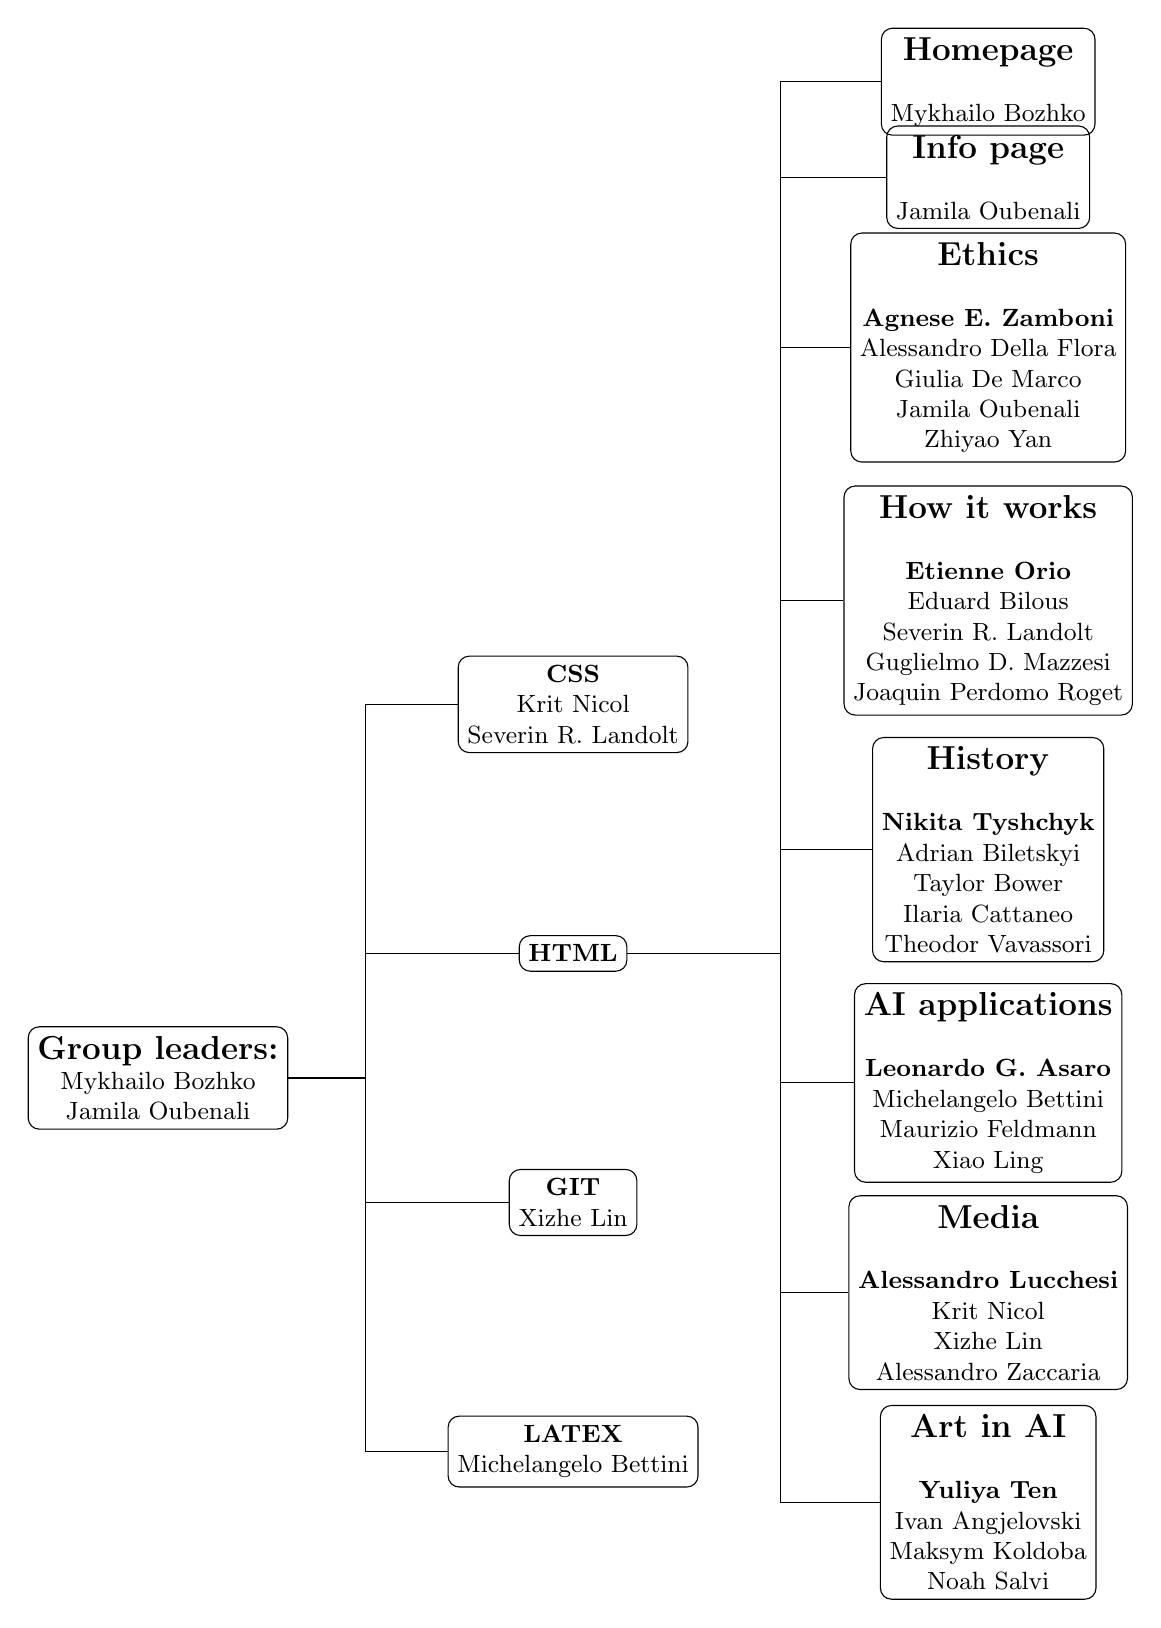
\begin{tikzpicture}
      [sibling distance=9em,level distance=15em,
      every node/.style={shape=rectangle,draw,rounded corners,align=center},
      edge from parent fork right,font=\small]
\node{\large{\textbf{Group leaders:}}\\Mykhailo Bozhko\\Jamila Oubenali}[grow=right]
    child{node[grow=right]{\textbf{LATEX}\\Michelangelo Bettini}}
    child{node[grow=right]{\textbf{GIT}\\Xizhe Lin}}
    child{node{\textbf{HTML}}
        child{node[yshift=4.1cm][grow=right]{\large{\textbf{Art in AI}}\\\\\textbf{Yuliya Ten}\\Ivan Angjelovski\\Maksym Koldoba\\Noah Salvi}}
        child{node[yshift=3.6cm][grow=right]{\large{\textbf{Media}}\\\\\textbf{Alessandro Lucchesi}\\Krit Nicol\\Xizhe Lin\\Alessandro Zaccaria}}
        child{node[yshift=3.1cm][grow=right]{\large{\textbf{AI applications}}\\\\\textbf{Leonardo G. Asaro}\\Michelangelo Bettini\\Maurizio Feldmann\\Xiao Ling}}
        child{node[yshift=2.9cm][grow=right]{\large{\textbf{History}}\\\\\textbf{Nikita Tyshchyk}\\Adrian Biletskyi\\Taylor Bower\\Ilaria Cattaneo\\Theodor Vavassori}}
        child{node[yshift=2.9cm][grow=right]{\large{\textbf{How it works}}\\\\\textbf{Etienne Orio}\\Eduard Bilous\\Severin R. Landolt\\Guglielmo D. Mazzesi\\Joaquin Perdomo Roget}}
        child{node[yshift=2.95cm][grow=right]{\large{\textbf{Ethics}}\\\\\textbf{Agnese E. Zamboni}\\Alessandro Della Flora\\Giulia De Marco\\Jamila Oubenali\\Zhiyao Yan}}
        child{node[yshift=1.95cm][grow=right]{\large{\textbf{Info page}}\\\\Jamila Oubenali}}
        child{node[grow=right]{\large{\textbf{Homepage}}\\\\Mykhailo Bozhko}}}
        child{node[grow=right]{\textbf{CSS}\\Krit Nicol\\Severin R. Landolt}};
   \end{tikzpicture}


 \subsection{Communication}
\begin{tabular}{p{12.3cm} p{4.7cm}}
 The Group uses a Discord server for official communications, which is divided into Categories with its own channels for every subject. There is also a summary of guidelines that should be respected by everyone while using git, and creating pages. Also all group members are encouraged to thoroughly track their sources, and make their commit messages as readable as possible. This communication method is integrated by also a Whatsapp group in case there was a need to reach out to an unresponsive teammate. 
 \newline\newline
  
\includegraphics[scale=0.338]{Git_comments.png}
 &
 \vspace{-0.5cm}
 \begin{flushright}

\includegraphics[scale=0.54]{DiscordServer.png}
 \end{flushright}\\
 \multicolumn{2}{c}{
\includegraphics[scale=0.405]{server-organization.png}}
\end{tabular}
\newpage

\section{Internal deadlines}
\small{Disclaimer: The internal deadlines may vary.}
\subsection{Before Monday 07.11}
\begin{itemize}[label=$\bullet$]
    \item Everyone researches their assigned subject and discusses it with their subject leaders to get an idea of what the topics will be. 
    \item The CSS team works on the CSS template, discusses the general appearance of the website with all the other group members to define all the needed features.
\end{itemize}

\subsection{Monday 07.11 \small{(20h00)}} 
\begin{itemize}[label=$\bullet$]
    \item The Subject leaders will submit a document with the structure of their website part and estimate how many pages their group might write for this.
    \item The Subject leaders will also communicate to the CSS team about their "design ideas", i.e. a general description of how their typical page layout may look like and what components will be used the most. 
\end{itemize}
What to work on after this deadline:
\begin{itemize}[label=$\bullet$]
    \item Every team member keeps researching their subjects.
    \item The Subject leaders and team members will have to expand the the topics proposed with more in-depth research. After that the teams will divide amongst them the workload.
    \item In the meantime the group leaders will organize the presentation for Friday 11.09.
\end{itemize}

\subsection{Wednesday 09.11}
\begin{itemize}[label=$\bullet$]
    \item Group meeting presenting the git repository to explain all members how to use it, and how to use the templates.
    \item {\footnotesize{(20h00)}} The CSS team must present the completed CSS file, and a few webpage templates.
    \item {\footnotesize{(20h00)}} The LaTeX team has to send the organization document to the Group leaders.
    \item {\footnotesize{(20h00)}} The Group leaders must send via email the address of the GIT repository.
\end{itemize}
 
\subsection{Friday 11.11}
\begin{itemize}[label=$\bullet$]
    \item The team leaders and group leaders meet up to review the feedback, talk about the final plan and smooth over the final details.
\end{itemize}

\subsection{Saturday 12.11}
\begin{itemize}[label=$\bullet$]
    \item All the group members should start writing their code.
\end{itemize}

\subsection{Thursday 17.11\small{(12h30)}}
\begin{itemize}[label=$\bullet$]
    \item All the group members must submit their code and start debugging it. 
    \item The team leaders should review the code of their team.
    \item {\footnotesize{(18h00)}} Meeting of the team leaders.
\end{itemize}

\section{Topics}

\subsection{Ethics}
\begin{itemize}[label=$\bullet$]
    \item \textbf{Ethics in Artificial Intelligence} - Agnese E. Zamboni
     \begin{itemize}[label=$\circ$]
         \item Introduction 
     \end{itemize}
    \item \textbf{Responsible A} - Alessandro Della Flora
     \begin{itemize}[label=$\circ$]
         \item What are ethics in AI, why is it important 
         \item Should AI replace job positions?
         \item Ethics of autonomous weapons
         \item The trolley problem with self-driving cars
     \end{itemize}
    \item \textbf{Explainable AI} - Agnese E. Zamboni
     \begin{itemize}[label=$\circ$]
         \item What is explainable AI (XAI), why is it important?
     \begin{itemize}
         \item Opaque artificial intelligence : black-box / white-box machine learning
         \item It is important to be able to explain the reason behind the decision of an AI machine to understand what it actually does
         \item Explainability tools
         \item Garbage-in garbage-out
     \end{itemize}
     \item Garbage-in garbage-out explanation and examples
     \end{itemize}
    \item \textbf{Data sets and Algorithmic bias} - Giulia De Marco
     \begin{itemize}[label=$\circ$]
         \item What are data sets and how it can be biased
         \item College admissions
         \item Apple face recognition works poorly with asian/black people
         \item COMPAS (correctional offender management profiling for alternative sanctions)
         \item Examples of bad data sets
     \end{itemize}
    \item \textbf{Misuse of AI} - Zhiyao Yan
     \begin{itemize}[label=$\circ$]
         \item What is it? how use of AI with bad intentions can be dangerous
         \item Deepfake
         \item Password Guessing
         \item Human Impersonation for monetary gain
         \item AI-supported hacking
     \end{itemize}
    \item \textbf{Initiatives to improve ethics in AI} - Jamila Oubenali
     \begin{itemize}[label=$\circ$]
         \item List of initiatives
     \end{itemize}
\end{itemize}

 \subsection{How it works}
 \begin{itemize}[label=$\bullet$]
     \item \textbf{"Vanilla" Neural networks} - Joaquin Perdomo Roget
     \begin{itemize}[label=$\circ$]
         \item Layers
         \item Activation functions
         \item Forwardpropagation
         \item Output layer functions
     \end{itemize}
     \item \textbf{Training} - Etienne Orio
     \begin{itemize}[label=$\circ$]
         \item Loss function
         \item Gradient descent
         \item Chain rule
         \item Backpropagation
     \end{itemize}     
     \item \textbf{Training techniques} - Guglielmo D. Mazzesi
     \begin{itemize}[label=$\circ$]
         \item Optimizers
         \item Initial weight values
         \item Regularization
         \item Validating Hyperparameters
     \end{itemize}     
     \item \textbf{Convolutional neural networks} - Eduard Bilous
     \begin{itemize}[label=$\circ$]
         \item Problem with fully connected layers
         \item Convolutional layer
         \item Pooling layer
         \item Visualizing a CNN
     \end{itemize}     
     \item \textbf{Natural Language Processing} - Severin R. Landolt
     \begin{itemize}[label=$\circ$]
         \item Introduction to NLP
         \item NLP Comparison
         \item Types of NLP
         \item The frontier of NLP
     \end{itemize}          
 \end{itemize}
 
 \newpage
 \subsection{History}
 \begin{itemize}[label=$\bullet$]
     \item \textbf{380 BC - 1950} | Nikita Tyshchyk
     \item \textbf{1950 - 1970} | Ilaria Cattaneo
     \item \textbf{1970 - 1990} | Adrian Biletskyi
     \item \textbf{1990 - 2010} | Taylor Bower
     \item \textbf{2010 - present} | Theodor Vavassori
     \item Famous people
     \begin{itemize}[label=$\circ$]
     \item[\ding{212}] Nikita Tyshchyk:\textbf{
         \item Cynthia Breazel
         \item Yutaka Matsuo
         \item Dacheng Tao
         \item Elon Musk}
         \item[\ding{212}] Ilaria Cattaneo:\textbf{
         \item Donald Olding
         \item Richard Socher
         \item Anita Schjøll Brede
         \item Anna Scaife
         \item Edward Feigenbaum}
         \item[\ding{212}] Theodor Vavassori:\textbf{
         \item Alan Turing
         \item Fei-Fei Li
         \item Rita Cucchira
         \item Jurgen Schmidhuber
         \item IBM(company)}
         \item[\ding{212}] Adrian Biletskyi:\textbf{
         \item Dorian Selz
         \item Demis Hassabis
         \item Andres Hardebring
         \item Robin Li
         \item Claude Elwood}
         \item[\ding{212}] Taylor Bower:\textbf{
         \item Rodney Brooks
         \item John McCarthy
         \item Martin Minsky
         \item Yann LeCun
         \item Ross Quillian}
     \end{itemize} 
 \end{itemize}
 
 \subsection{AI applications in the field}
 \begin{itemize}[label=$\bullet$]
     \item[\ding{212}] Xiao Ling:
     \item \textbf{Trading}
     \begin{itemize}[label=$\circ$]
         \item Support Vector Machines
         \item Artificial Neural Networks in the stock markets
         \item Technical Analysis and Pattern Recognition as aid to investors
         \item Algorithmic trading
         \item High Frequency Trading
     \end{itemize}
     \item \textbf{Education}
     \begin{itemize}[label=$\circ$]
         \item Differentiated and individualized learning offered by AI
         \item Universal access to lectures for students of different nationalities
         \item Technical Analysis and Pattern Recognition as aid to investors
         \item Automation of admin tasks
         \item Tutoring and support outside the class
     \end{itemize}
     \item[\ding{212}] Leonardo G. Asaro:
     \item \textbf{Self-driving vehicles}
     \begin{itemize}[label=$\circ$]
         \item Self-driving cars
         \item Autonomous flight
     \end{itemize}
     \item \textbf{Traffic data analysis}
     \begin{itemize}[label=$\circ$]
         \item Google Maps' traffic analysis
         \item AI in traffic management
     \end{itemize}
     \item[\ding{212}] Michelangelo Bettini:
     \item \textbf{Factory Automation}
          \begin{itemize}[label=$\circ$]
         \item Forecast of errors and disruptions
         \item AI trained image recognition for quality checks (citation to Quality Control)
         \item Use of AGVs (autonomous guided vehicles) inside factories
         \item Use of AI for generative design
         \item Reduce waste and costs whilst being more efficient
     \end{itemize}
     \item \textbf{Quality Control}
     \begin{itemize}[label=$\circ$]
         \item Visual Inspection AI by Google, applied in different fields
     \end{itemize}
     \item \textbf{Warehouse Management}
     \begin{itemize}[label=$\circ$]
         \item Inventory management
         \item Material handling
         \item Processing and packaging
         \item Supply chain
         \item Demand planning
     \end{itemize}
     \item[\ding{212}] Maurizio Feldmann:
     \item \textbf{Medicine}
          \begin{itemize}[label=$\circ$]
         \item Improve diagnostics
         \item Manage population health
         \item Accelerate drug discovery
         \item modernize care Infrastructure
     \end{itemize}
     \item \textbf{Cybersecurity}
     \begin{itemize}[label=$\circ$]
         \item Threat detection
         \item Breach Risk Prediction
         \item Advantages of using AI in this field
         \item Automation of bot detection
         \item Behaviour profiling
         \end{itemize}

 \end{itemize}

\subsection{Media} 
\begin{itemize}[label=$\bullet$]
    \item \textbf{Introduction} - Alessandro Lucchesi
    \item \textbf{Marketing} - Krit Nicol | Xizhe Lin
    \begin{itemize}[label=$\circ$]
        \item How it's used
        \item Examples
        \item Use in dating apps
        \item Use in song streaming
     \end{itemize}
    \item \textbf{Politics} - Alessandro Lucchesi 
    \begin{itemize}[label=$\circ$]
         \item Cambridge Analytica scandal
         \item Malicious software using social media
     \end{itemize}
     \item \textbf{Examples} - Alessandro Zaccaria
    \begin{itemize}[label=$\circ$]
         \item Linkedin social experiment 
     \end{itemize}
          \item \textbf{How it's changing traditional media} - Xizhe Lin
    \begin{itemize}[label=$\circ$]
         \item Automated journalism
     \end{itemize}
\end{itemize}

\newpage
 \subsection{Art in AI}
 \begin{itemize}[label=$\bullet$]
     \item \textbf{Images} - Yuliya Ten
      \begin{itemize}[label=$\circ$]
          \item Creating
          \item Editing
          \item NFT
      \end{itemize}
      \item \textbf{Videos} - Ivan Angjelovski
        \begin{itemize}[label=$\circ$]
          \item 4D stuntman
          \item AI based films
       \end{itemize}
      \item \textbf{Literature} (NLP)Now - Ivan Angjelovski
      \item \textbf{Music} - Noah Salvi
      \begin{itemize}[label=$\circ$]
          \item Voice alteration
      \end{itemize}
      \item \textbf{Games} - Maksym Koldoba
      \begin{itemize}[label=$\circ$]
          \item RTX + DLSS
      \end{itemize}
 \end{itemize}


\section{GIT repository structure}
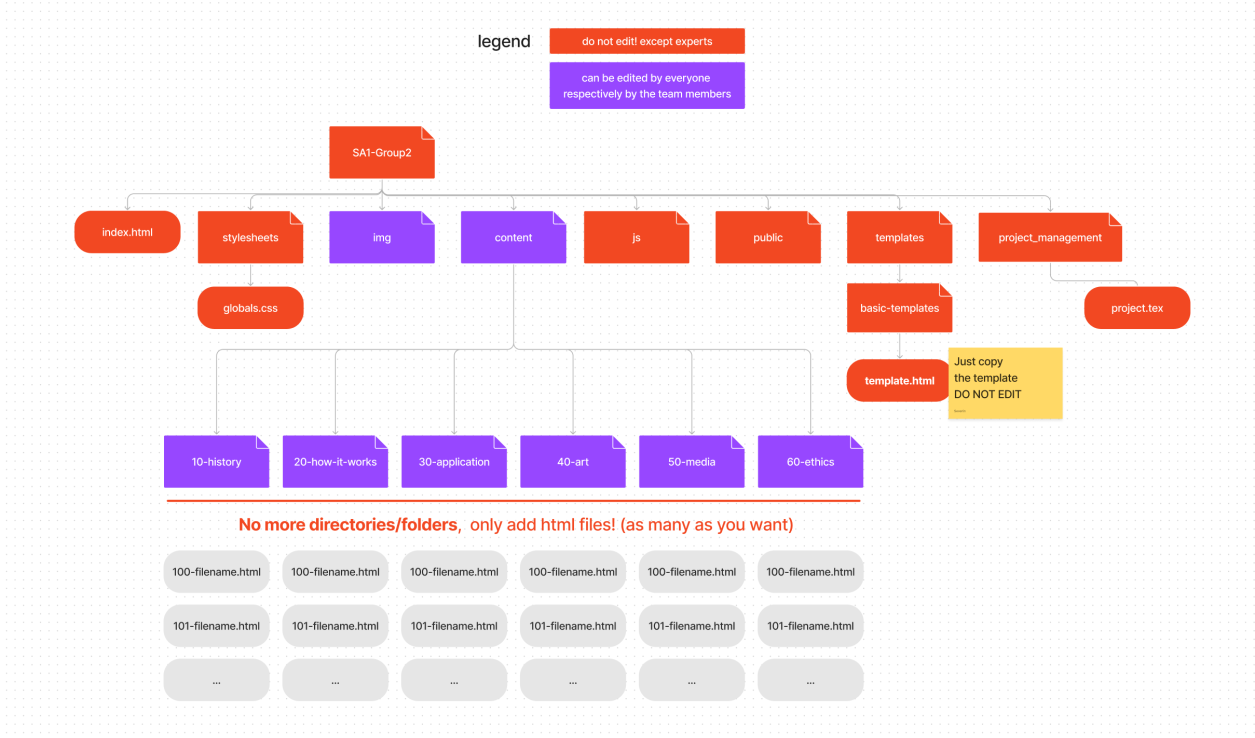
\includegraphics[width=\linewidth]{GITRepStr.png}
\section{Template page}
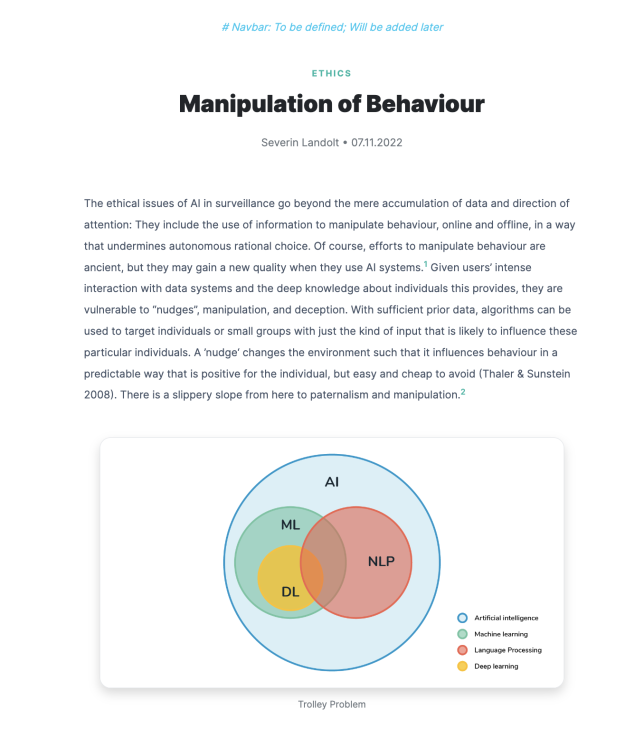
\includegraphics[width=\linewidth]{templatepage.png}
\section{HTML \& CSS example}
\begin{center}

\includegraphics[width=345px]{Templstepage_html.png}\\
\vspace{1em}
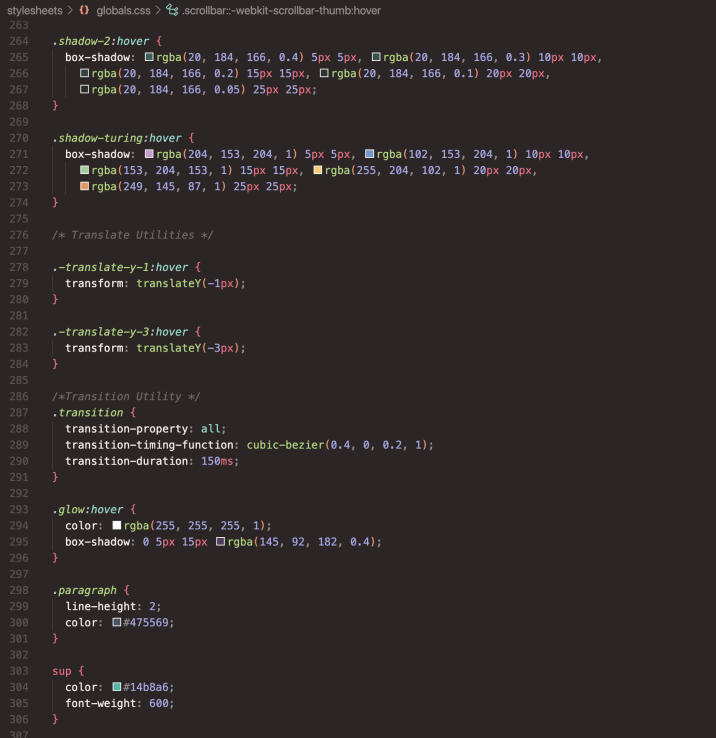
\includegraphics[width=345px]{CSScode.png}
\end{center}

\end{document}
